\documentclass{article}
\usepackage{iclr2027_conference,times}
\input{math_commands.tex}
\usepackage{hyperref}
\usepackage{url}
\usepackage{booktabs}
\usepackage{multirow}
\usepackage{graphicx}
\usepackage{xcolor}
\usepackage{enumitem}
\usepackage{algorithm}
\usepackage{algpseudocode}
\usepackage{tikz}
\usetikzlibrary{arrows.meta,positioning,shapes.misc,calc}
\usepackage{pgfplots}
\pgfplotsset{compat=1.18}
\usepackage{caption}
\captionsetup{skip=4pt}
\setlength{\textfloatsep}{8pt plus 2pt minus 2pt}
\setlength{\intextsep}{6pt plus 2pt minus 2pt}
\setlength{\abovecaptionskip}{4pt}
\usepackage{microtype}
\usepackage{xspace}

\setlist{nosep,leftmargin=1.3em}
\newcommand{\bpt}{Blair et al.\xspace}
\newcommand{\sys}{Freedi\xspace}
\newcommand{\pass}[1]{\textsc{p#1}}
\newcommand{\hl}[1]{\textbf{#1}}
\hypersetup{colorlinks=true,linkcolor=blue!60!black,citecolor=blue!60!black,urlcolor=blue!60!black}

% Uncomment for the camera-ready version.
% \iclrfinalcopy

\title{Geometry Proposes, Judgement Disposes:\\Engineering Online Claim Aggregation for Live Deliberation}

\author{Tal Yaron \\
Freedi \\
\texttt{tal.yaron@wizcol.com}
\And
Nimrod Talmon \\
Ben-Gurion University of the Negev \\
\texttt{talmonn@bgu.ac.il}
\AND
Erel Segal-Halevi \\
Ariel University \\
\texttt{davidesh@ariel.ac.il}
\And
Fany Yuval \\
Ben-Gurion University of the Negev \\
\texttt{fanyuval@bgu.ac.il}
}

\begin{document}

\maketitle

\begin{abstract}
Online deliberation platforms ask participants an open question and collect the answers as free text. Fifty people who ask for the same thing in fifty wordings then look like fifty minority positions. The platform must therefore decide, for each new statement and while the deliberation is running, whether the statement repeats an existing proposal, relates to one, or is new. This paper describes the engine that makes that decision in a deployed platform, and the one rule the engine converged on after a year of measured failures: \emph{embedding similarity may propose candidates, but it may never decide}. Every placement that changes what the public sees is a discrete, cached, fail-closed judgement by a language model over the actual texts, and an optional \emph{claim registry} turns deduplication into classification against a growing codebook of canonical claims. We evaluate the engine on three instruments. On the 875 hard preference triplets of \bpt (2026), our production embedding scores 0.5\% and lets almost every stance-flipped distractor through every merge threshold, while the judged registry scores 95.0\%, against 80--81\% for the best repaired geometry. On a 100-statement corpus streamed through the live trigger path, the synthesis layer recovers all 150 ground-truth pairs across three arrival orders with no false merge. On a replayed production question, blind auditors measure merge precision of 74\%, and we report that number rather than the benchmark one. We then test the obvious alternative: a language model with no pipeline at all. On the clean corpus it is just as exact and organises themes better, so the pipeline earns its keep through scale, streaming and cost, not per-decision accuracy. Where the bare model does fail is at scale: it drops from 95\% to 36--56\% on long candidate lists, drifts across model upgrades, converges to spurious merges when asked repeatedly, and hides outages inside its verdicts. We close with the failure modes that shaped the design and with how our decision layer composes with \bpt's preference geometry.
\end{abstract}

\section{Introduction}

A growing family of systems asks people to express their views as free text rather than as votes on a fixed slate. Polis \citep{small2021polis}, Remesh, the Habermas Machine \citep{tessler2024ai} and generative social choice \citep{fish2026generative,boehmer2025generative} all belong to it, and all of them need the same primitive: given many free-form statements, decide which ones say the same thing. Two shortcuts present themselves. The first embeds each statement and merges whatever lies within a cosine threshold. The second hands the whole corpus to a large language model and asks for groups. We run a deliberation platform that has had to answer this question in production, for tens of thousands of statements in English and Hebrew, and this paper reports what we learned. Both shortcuts fail, for different reasons, and the architecture that works is neither.

The geometric shortcut fails for a reason \bpt \citeyearpar{blair2026embeddings} make formal. An off-the-shelf embedding encodes the stance of a statement entangled with its topic, wording and style. On natural data the two are correlated, so cosine similarity appears to track stance, and it keeps appearing to until the correlation is deliberately broken. Their remedy is to repair the geometry. Ours, reached independently from production incidents, is to demote it. The two remedies can be compared directly, because we benchmarked our decision layer on the hard-triplet set they released (\S\ref{sec:triplets}).

The LLM shortcut fails less visibly, and we want to be exact about what fails. A language model is an excellent judge of a pair of statements, or of a short list of candidates. On a clean corpus small enough to fit in one prompt it is also an exact clustering algorithm, and we show this with our own benchmark (\S\ref{sec:llmonly}). What breaks is the operating regime of a live system. Accuracy collapses as the candidate list grows (\S\ref{sec:whynotllm}). Free-form canonical wordings drift from one model generation to the next (\S\ref{sec:pilot}). A model asked repeatedly to ``find groups'' in an unchanging set eventually proposes a wrong merge, and a live system asks it every ten minutes (\S\ref{sec:convergence}). The cost of placing each arrival against the whole corpus grows quadratically. And every one of these failures is silent unless the system is built to tell an outage from a verdict.

\paragraph{Contributions.}
(1) A production architecture for \emph{online} claim aggregation in which geometry only proposes candidates and every placement is a discrete, cached, fail-closed judgement (\S\ref{sec:system}). (2) The \emph{claim registry}, which treats deduplication as classification against a growing per-question codebook, with consolidation, a mutation protocol, self-audit counters and typed \emph{opposes} edges that no metric can represent (\S\ref{sec:registry}). (3) An evaluation on \bpt's 875 hard triplets, on a live end-to-end benchmark in two languages, on a replayed production question with blind audit, and against LLM-only baselines (\S\ref{sec:eval}). (4) A catalogue of the failure modes of embedding-threshold clustering, each with the structural change that answered it (App.~\ref{app:failures}). (5) An argument that our decision layer and \bpt's preference geometry are complementary, and a concrete hybrid (\S\ref{sec:bpt}).

\section{Problem Setting}
\label{sec:problem}

Participants answer an open question, for example \emph{``What should our city do to improve residents' quality of life?''}, with short proposals, and they rate each other's proposals on a continuous scale. The engine has three jobs, and it does all three continuously. \textbf{Synthesis}: notice that two statements make the \emph{same proposal} in different words, and replace them with one jointly worded statement that pools their ratings. \textbf{Theming}: group proposals that are related but distinct under a topical heading, without pretending they agree. \textbf{Standing}: leave everything else alone, visibly, from the first statement onward.

Stated formally, statements $x_1, x_2, \dots$ arrive in an order we do not control. The state $S_t$ is the set of clusters built so far, syntheses and themes, over $\{x_1..x_{t-1}\}$. The unit of work is: \emph{given $x_t$ and $S_t$, decide where $x_t$ belongs}. This is an online placement problem, not a one-shot clustering problem, and four constraints shape every design choice. The decision must be made live, within seconds, with no batch step a user waits for. The arrival order must not change what people end up agreeing to. Corpora are per question, between a hundred and ten thousand statements, in several languages. And spending on language-model calls must be bounded and auditable.

Two distinctions carry most of the conceptual weight. \emph{Same topic is not same proposal}: ``add speed bumps near schools'' and ``lower the speed limit near schools'' share a goal but are different interventions, and merging them misrepresents both authors. \emph{Same words are not same stance}: ``ban X'' and ``do not ban X'' are nearly identical as strings and opposite as positions. The two kinds of error are not symmetric. A wrong merge files a statement under a proposal its author would reject, silently and permanently, for every reader. A missed merge leaves a visible duplicate that a later sweep can repair. Every tie-breaking rule in the system leans toward the repairable error.

\section{Why Neither Geometry Nor a Bare LLM Suffices}
\label{sec:why}

\subsection{Geometry: a topicality signal wearing a preference costume}
\label{sec:whynotgeom}

\bpt decompose the cosine margin between an anchor $a$, a preference match $p$ and a semantic distractor $n$ into a stance component and a nuisance component, $s(a,p)-s(a,n)=\Delta_S+\Delta_T$, and observe that cosine weights the two equally. On a \emph{hard triplet}, where the distractor keeps the anchor's wording and flips its stance, the nuisance dominates, and base encoders rank the distractor above the match 52--94\% of the time. Our production measurements say the same thing from the other side (Table~\ref{tab:triplets}). With our production embedding, \hl{every stance-flipped distractor clears the pipeline's topical gate of 0.60, and 99.1\% clear its strictest merge gate of 0.85}. The median distractor cosine, 0.969, sits \emph{above} the median match cosine, 0.871. A threshold that admits every counterfeit is not a weak classifier. It is not a classifier.

Three further facts from production make the problem worse. First, we embed every statement under a shared question prefix, and the prefix lifts the whole cosine floor: on our live corpus, 80\% of English and 100\% of Hebrew \emph{cross-topic} pairs sit above 0.60. Second, thresholds belong to a geometry, not to a pipeline: when we upgraded the Hebrew embedding model without recalibrating the bands, a failure we had already fixed came back (App.~\ref{app:failures}). Third, theme membership is not in the geometry at all. The best single cosine cut over ground-truth synthesis centroids reaches a topic F1 of 0.48; moving that decision to a judge took it to 0.78.

And yet nearest-neighbour search over the same embeddings reliably \emph{finds} the true partner. The paraphrase twin is the top neighbour for 100 of 100 English statements, and at a retrieval floor of 0.45 no true match was lost in any language we tested (\S\ref{sec:recallgap}). Geometry knows what is \emph{relevant} even when it cannot tell \emph{which side}. That asymmetry is the whole design.

\subsection{A bare LLM: an excellent judge, a poor clustering algorithm}
\label{sec:whynotllm}

The natural reaction is to skip geometry and let a language model decide everything. On a corpus small enough to fit in one prompt, this works, and \S\ref{sec:llmonly} says so with numbers. What follows is why it does not survive the production regime.

\emph{Scale and cost.} Judging every pair of $n$ statements costs $\Theta(n^2)$ calls. One of our own scheduled sweeps lacked a spend bound on refusals and cost about 3{,}100 completions a day on proposals nobody was touching (\S\ref{sec:cost}). Placing each arrival against the whole corpus costs $\Theta(n)$ tokens per arrival and $\Theta(n^2)$ overall, and it is bounded by the context window. One-shot batch clustering has no online form at all: rebuilding the groups on every arrival can change what earlier participants already agreed to.

\emph{Long lists.} The judge that scores 95.0\% against a single candidate claim scores 36--56\% under strict scoring when it must choose among a codebook of about 94 claims (Table~\ref{tab:triplets}). This matches what is known about position bias and long contexts \citep{liu2024lost,wang2023large}. A judge over a short ranked list and a judge over a long one are not the same instrument.

\emph{Unstable canonical wordings.} One might ask the model to write a ``simple meaning'' sentence for each statement and compare those. This recreates the problem one level up: two calls canonicalise the same idea in two different ways. Classification into a fixed set converges; free-form generation does not. Even with the codebook fixed, replacing raw text with a generated canonical wording cost 24.9 points of accuracy (95.0\% to 70.1\%), and a later model upgrade cost the enriched-canonical configuration a further 12 points while leaving raw-text classification untouched (\S\ref{sec:pilot}).

\emph{Silent failure.} A rate limit that is exhausted and ``fails closed'' to \emph{none} looks exactly like a burst of honest verdicts saying ``this is new''. In one of our runs, 260 of the first 456 classifications were this kind of silent corruption. Reasoning models add a second route: on some inputs they spend the whole completion budget on hidden reasoning and return empty output, deterministically. Outages must therefore be tracked apart from verdicts, fallback verdicts must never be cached, and every action the system drops must have a custodian. Two further hazards, non-determinism under repeated judgement and sensitivity to prompt wording, are documented in App.~\ref{app:llmhazards}. Finally, a batch partition is a fait accompli, whereas participants are entitled to a stated reason and a typed relation for every placement.

The conclusion is not ``do not use a language model''. It is a division of labour. Geometry proposes a short, ranked candidate set. The model disposes, with a discrete verdict over the texts, under a doubt bias that leans toward the repairable error, failing closed, cached, budgeted on cache misses, and logged with its reason.

\section{The System}
\label{sec:system}

\begin{figure}[t]
\centering
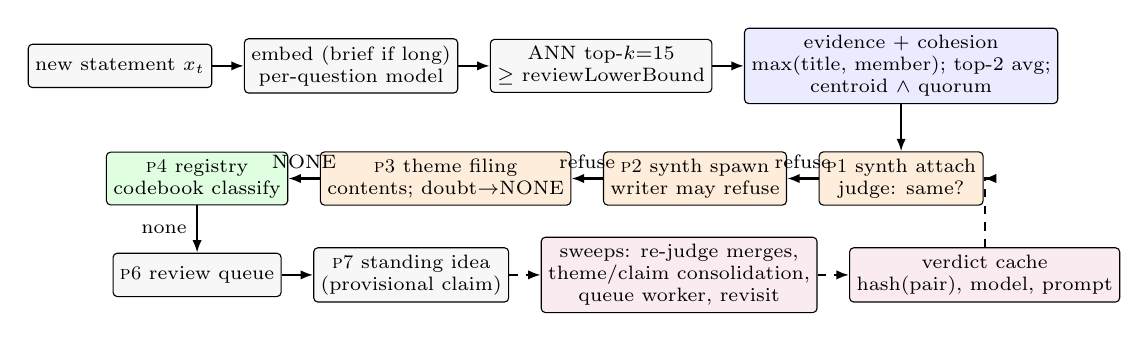
\begin{tikzpicture}[
  font=\scriptsize, node distance=3mm and 4mm,
  box/.style={draw, rounded corners=1.5pt, align=center, inner sep=2.5pt, minimum height=5.5mm, fill=gray!6},
  gate/.style={box, fill=blue!8},
  judge/.style={box, fill=orange!14},
  reg/.style={box, fill=green!12},
  arr/.style={-{Latex[length=1.6mm]}, thick}
]
\node[box] (in) {new statement $x_t$};
\node[box, right=of in] (emb) {embed (brief if long)\\per-question model};
\node[box, right=of emb] (ann) {ANN top-$k{=}15$\\$\ge$ reviewLowerBound};
\node[gate, right=of ann] (ev) {evidence + cohesion\\max(title, member); top-2 avg;\\centroid $\wedge$ quorum};
\node[judge, below=6mm of ev] (p1) {\pass{1} synth attach\\judge: same?};
\node[judge, left=of p1] (p2) {\pass{2} synth spawn\\writer may refuse};
\node[judge, left=of p2] (p3) {\pass{3} theme filing\\contents; doubt$\to$NONE};
\node[reg, left=of p3] (p4) {\pass{4} registry\\codebook classify};
\node[box, below=6mm of p4] (p6) {\pass{6} review queue};
\node[box, right=of p6] (p7) {\pass{7} standing idea\\(provisional claim)};
\node[box, right=of p7, fill=purple!8] (sw) {sweeps: re-judge merges,\\theme/claim consolidation,\\queue worker, revisit};
\node[box, right=of sw, fill=purple!8] (vc) {verdict cache\\hash(pair), model, prompt};
\draw[arr] (in) -- (emb); \draw[arr] (emb) -- (ann); \draw[arr] (ann) -- (ev);
\draw[arr] (ev) -- (p1);
\draw[arr] (p1) -- node[above]{refuse} (p2);
\draw[arr] (p2) -- node[above]{refuse} (p3);
\draw[arr] (p3) -- node[above]{NONE} (p4);
\draw[arr] (p4) -- node[left]{none} (p6);
\draw[arr] (p6) -- (p7);
\draw[arr, dashed] (p7) -- (sw);
\draw[arr, dashed] (sw) -- (vc);
\draw[arr, dashed] (vc.north) |- ($(p1.east)+(0,0)$);
\end{tikzpicture}
\caption{The placement cascade. Blue boxes are geometric gates, which only decide candidacy. Orange boxes are language-model judgements, the only steps that change what the public sees. Green is the optional registry; purple is the convergence layer. A statement takes the first pass whose gate \emph{and} judgement both admit it.}
\label{fig:arch}
\end{figure}

\subsection{Representation and retrieval}
We embed statements with OpenAI's \texttt{text-embedding-3-small} at 1536 dimensions \citep{openai2024embeddings}. A stronger model, \texttt{-3-large} truncated to the same width, can be pinned \emph{per question}, because vectors from two models live in different spaces and a cosine between them means nothing. Hebrew forces the pin: under the small model the paraphrase twin is the nearest neighbour for only 56 of 100 Hebrew statements, against 100 of 100 in English; under the large model it is 88--89 of 100. Long statements are first distilled into a five-to-fifteen-word \emph{brief}, and the brief is what we embed, because boilerplate otherwise makes everything look about 0.75 similar to everything else. Candidates come from approximate nearest-neighbour search within the question, top $k=15$. We raised $k$ from 10 after compressed Hebrew geometries buried true partners below rank 10. Cosine values are partitioned into calibrated bands (App.~\ref{app:bands}) that obey $\text{review}<\text{cluster}\le\text{synthLower}\le\text{attach}$. Crossing a band makes a statement a \emph{candidate} for an action. It never triggers the action.

\subsection{Evidence and cohesion gates}
\label{sec:cohesion}
The evidence for a candidate cluster is deliberately not ``similarity to the cluster's title''. A merged title abstracts away from its members, so title-only evidence spawns duplicate clusters. But the opposite rule, title \emph{or} any single member, lets a cluster \emph{snowball}: a newcomer that paraphrases one member joins, the next newcomer paraphrases a different member and joins too, and the cluster ends up spanning several ideas held together by a chain of pairwise links. We saw exactly this in production, when one synthesis absorbed four unrelated proposals, the last of them at cosine 0.43 to the rest.

We therefore separate discovery from admission. For discovery, a cluster's candidacy is the maximum of its title cosine and its best member cosine. For admission, we fetch every member's embedding and score the cluster by the \emph{average of its two highest member cosines}, so that two independent members must agree; and we track member-only evidence separately, so the strictest gate can demand agreement with the cluster's contents rather than its label. Before any merge candidate reaches a judge, the receiving cluster must also pass a cohesion gate: the newcomer must be close to the member centroid \emph{and} broadly related to at least half the members. The centroid floor, 0.815 at default bands, comes from a measured separation over 4{,}900 candidates, where genuine attaches had a median centroid cosine of 0.898 and false same-topic candidates a median of 0.723. We first built this gate as an OR with lower floors, and in a 100-statement run it refused nothing. The conjunction is what makes it a brake.

\subsection{The placement cascade}
\label{sec:cascade}
Algorithm~\ref{alg:cascade} gives the decision tree. One function serves all five entry points (live creation, threshold crossings, the retry queue and two admin actions), and that is what makes the behaviour analysable. Three ordering rules matter, and each was learned from a measured failure.

\emph{Most specific first.} Synthesis passes run before theming, because a theme that already holds your twin will always look cohesive to you: your twin is inside its centroid. When theming ran first, 17 of 23 topical attachments in one run were justified by the statement's own paraphrase twin, and only 2 of 50 ground-truth pairs ever merged: the pipeline was using the twin as evidence to file the statement away from it.

\emph{Topic membership is not terminal.} A statement owned by a theme has been given a theme, not a meaning, and it stays eligible for synthesis when its twin arrives. Treating the first cluster to touch a statement as its permanent owner was the largest single source of missed pairs. Synthesis membership \emph{is} terminal, and an authoritative reverse-membership query enforces exactly one owner even when the queue replays an item.

\emph{Judge every attach.} The first pass was the last placement that acted on geometry alone. Under Hebrew with the large model, distinct transport proposals attached to one synthesis at cosines of 0.899--0.944, above every gate, because in that space distinct ideas and paraphrases are geometrically indistinguishable. The equivalence judge now gates that pass too, cached and fail-closed. An unmerged duplicate heals itself through the sweep; a wrong attach is permanent.

\begin{algorithm}[t]
\caption{Online placement of one statement (abridged; every pass fails closed on a judge error).}
\label{alg:cascade}
\begin{algorithmic}[1]
\scriptsize
\State $e \gets \textsc{Embed}(x_t)$; $C \gets \textsc{ANN}(e, k{=}15, \ge\text{reviewLowerBound})$
\If{$C=\emptyset$} \Return \textsc{Registry}$(x_t)$ \textbf{or} provisional singleton claim \EndIf
\State $E \gets$ best evidence per cluster: $\max(\text{title},\text{member})$, promoted to top-2 member average
\ForAll{synth $s$ with $E[s]\ge\text{attach}$, sorted desc} \Comment{\pass{1}}
  \State \textbf{if} member evidence $<$ attach \textbf{or} $\neg$\textsc{Cohesion}$(s,e)$ \textbf{then continue}
  \State \textbf{if} \textsc{JudgeCached}$(x_t, s)=\textsc{same}$ \textbf{then} attach; re-home theme; \Return
\EndFor
\ForAll{plain $y\in C$ in synth band, not in a synth, first 3} \Comment{\pass{2}}
  \State $r \gets \textsc{Writer}(x_t,y)$; \textbf{if} spawned \textbf{then} nest under theme; \Return
  \State \textbf{if} debounced \textbf{or} error \textbf{then} enqueue retry; \Return \Comment{never drop}
\EndFor \Comment{refusal: try next candidate}
\State \textbf{if} not in a theme: $\theta \gets \textsc{ThemeJudge}(x_t,\text{themes with contents})$; \textbf{if} $\theta\ne\textsc{none}$ attach; \Return \Comment{\pass{3}}
\State \textbf{if} registry on: $r\gets$\textsc{Classify}$(x_t,\text{codebook ordered by cosine})$; record \textsc{opposes} edge; \textbf{if} \textsc{expresses}$\wedge$conf$\ge$0.6 attach; \Return \Comment{\pass{4}}
\State queue $(x_t, \text{top}(C))$ for review \Comment{\pass{6}; resolved automatically if later placed}
\end{algorithmic}
\end{algorithm}

\subsection{The judges}
\label{sec:judges}
Every action that changes what the public sees is a language-model judgement over the actual texts, and every judge shares three safety properties. The first is \emph{asymmetric doubt}: each prompt carries an explicit tie-break toward the cheaper error. The equivalence judge is told that when in doubt between \emph{same} and \emph{related} it should prefer \emph{related}; the writer, that when in doubt it should refuse; the theme judge inverts the bias, because a topic created too eagerly is cheap while a proposal filed under the wrong topic stays there for every reader. The second is \emph{fail closed on placement, fail open on custody}: a judge error on a merge decision defaults to \emph{different}, a judge error while re-validating an existing cluster keeps its members, and outages are recorded apart from negative verdicts. The third is that the live path is conservative and the scheduled sweeps supply the convergence, so a live mistake is one of omission, and omissions are repaired by sweep.

The \textbf{equivalence judge} returns one of four verdicts, \textsc{same}, \textsc{related}, \textsc{different} or \textsc{opposite} (App.~\ref{app:prompts}). Only \textsc{same} merges. \textsc{opposite} is a typed relation that no distance function can represent, and the registry stores it as an edge.

The \textbf{synthesis writer} produces the joint statement, but its first task is a refusal check with two triggers: the inputs pull opposite ways on the same lever, or they are distinct actions within one theme. Two amendments to the rubric each came from a measured error. A \emph{formulation clause} tells the writer to refuse only when the difference \emph{is} the intervention, not when one input names a category and the other an instance of it; this took Hebrew twin recovery from 45 to 49 of 50 offline and changed no English verdict. A \emph{never-widen-scope rule} came after we found synthesised texts drifting toward helpful generalisation, turning ``freelancers'' into ``residents''. That drift silently changes what people are agreeing to. After the rule, scope inflation fell from 4 of 50 syntheses to none, and a fidelity audit over live runs found all 98 member intents preserved (App.~\ref{app:fidelity}). The writer's output language is forced by script detection, because titles are themselves embedded and reused as evidence, so a title in the wrong language is a retrieval corruption rather than a display bug.

The \textbf{theme judge} files a statement into an existing theme, may answer NONE, and never creates a theme. It is shown each theme's \emph{contents}, never its title alone, and it is told to answer NONE when unsure. The two ingredients only work together: contents under an eager bias made misfiling worse, and caution without contents made the judge refuse half of everything. Together they halved permanent misfiles live, from 20.7\% to 9.3\%. We chose among variants by a rule registered in advance, three times the misfiles plus the over-refusals, and rejected two variants with higher raw accuracy because they bought it by re-licensing misfiles (App.~\ref{app:filing}). Accuracy is the wrong objective for a decision whose two errors cost different amounts.

\subsection{The claim registry}
\label{sec:registry}
The cascade has a structural blind spot: the judge can rule only on pairs that cosine surfaced. Two statements with the same meaning but distant embeddings are never compared, and no threshold tuning can close that gap, because the failing pair never becomes a candidate. A second problem is cold start: cosine bands are calibrated on the density of mature questions and mean little when a question has five statements. The registry answers both with one move. It treats deduplication as \textbf{classification against a shared, growing codebook of canonical claims}, one per idea already seen in this question, each carrying a short canonical wording, a public explanation and a verbatim exemplar. Because claims are short, one call to a fast model reads \emph{all} of them, so recall no longer depends on geometry. Because classification is into a fixed set, canonical forms converge instead of drifting. And because meaning-judgement needs no calibration, the registry works as well at the second statement as at the two-thousandth. The classifier sees enriched lines, since bare canonical wordings cost 25 points (\S\ref{sec:triplets}), and it carries the stance caution learned from the hard triplets: shared phrasing is never evidence of a match. Cosine is demoted from gatekeeper to \emph{ranker}: it orders the codebook so that likely matches come first, which mitigates position bias, and it filters nothing. A statement that matches nothing spawns a one-member \emph{provisional} claim, so every idea is a labelled public idea from the moment it exists.

The registry also maintains its codebook, because a codebook that drifts is worse than none. \emph{Consolidation} runs every fifteen placements: one call over the whole codebook proposes merges and flags claims that have grown too broad, under a rubric that says same-topic-different-action is not a merge and that no merge is a perfectly good answer. Each claim joins at most one merge per pass, membership transfers transitively, splits go to a human queue, and a claim is confirmed only once it has three members and has survived a pass untouched. A \emph{mutation protocol} classifies any rewording of a claim as reword, broaden, narrow or different, failing closed to \emph{different}, which forces one batched re-validation of the members. Because individually harmless broadenings compose, every claim keeps its original \emph{anchor text}, and after two unchecked broadenings the new wording is tested against the anchor. \emph{Self-audit} comes for free: every consolidation merge is, by construction, a case where the registry once said ``new'' and was wrong, so the running merge count estimates the registry's own recall error, a quantity that is otherwise invisible. Five percent of classifications are also re-run on a stronger model and logged, without overriding the decision. Above thirty claims, classification \emph{routes} through at most two topic claims, but any \textsc{none} triggers a full flat fallback, on the principle that a gate which filters can misfile while a gate with an ungated second look cannot. In a corpus replay, hard partitioning without that fallback caused 59\% of all recall loss, and adding the fallback moved accuracy from 61.3\% to 75.3\% ($p=7.5\times10^{-4}$). The registry is opt-in per question; the judged cascade is the default.

\subsection{Convergence and cost control}
\label{sec:convergence}
The live path optimises for latency and safety; scheduled functions supply eventual consistency (App.~\ref{app:convergence}). A queue worker drains deferred work every minute, and nothing may be dropped without an audit record or a scheduled second chance. A re-judge sweep proposes cross-synthesis merges wherever the member evidence across two syntheses exceeds 0.82, a value deliberately \emph{below} decision grade because the two relevant bands overlap there; the judge confirms each proposal, and the \emph{farthest} cross-member pair must also be judged \textsc{same}. Consolidation of themes and claims judges on \emph{members}, never on titles, and each distinct set of headings is judged \emph{once}, keyed on a fingerprint, so that a settled question is not put to a non-deterministic model 144 times a day.

\label{sec:costctl}
Four mechanisms bound the spending. A \emph{verdict cache} is keyed by an order-independent hash of the pair's texts and versioned by model and prompt; fallback verdicts from failures are never written, so a transient outage cannot poison later runs, and a cache hit costs about 45 milliseconds against about 2.3 seconds for a completion. \emph{Budgets are billed on cache misses only.} The sweep's per-question allowance counts judge calls rather than successful merges, because refusals cost a call and the old counter left the loop with no spend bound at all; and it counts only misses, because billing hits would spend the whole allowance on known answers and stall merging on the largest questions. Judge calls are \emph{batched}, twenty pairs per call and one call per cluster re-validation. And a fail-closed/fail-open policy table (App.~\ref{app:bands}) marks \texttt{failedClosed} as a first-class outcome, so a saturated rate limit looks like an outage and not like a burst of new ideas. In practice the engine costs about \$0.2--0.5 per thousand statements at one to two seconds per placement (App.~\ref{app:cost}).\label{sec:cost}

\section{Evaluation}
\label{sec:eval}

\subsection{Hard triplets: a shared instrument with \bpt}
\label{sec:triplets}
\bpt release 875 hard triplets drawn from eleven datasets on Polis, Remesh and generative-social-choice surveys. For each real participant anchor there is a \emph{match}, a same-stance paraphrase, and a \emph{distractor}, a stance-flipped rewrite that preserves the wording. Their metric is a ranking: $s(a,p)>s(a,n)$. Ours is stricter and end-to-end. A triplet counts as correct only if the match \emph{attaches} to the anchor's claim (verdict \textsc{expresses} at confidence $\ge0.6$) and the distractor does not. The harness imports the production functions unmodified. Intervals are Wilson 95\%, and paired contrasts use exact McNemar tests.

\begin{table}[t]
\centering\scriptsize
\caption{Triplet accuracy on the 875 hard triplets of \bpt. Paper rows are the authors' reported cosine accuracies; \sys rows are end-to-end attach decisions. McNemar, registry against raw cosine: 827 discordant wins to 0.}
\label{tab:triplets}
\resizebox{\linewidth}{!}{\begin{tabular}{@{}llr@{}}
\toprule
Condition & Decision mechanism & Acc.\ [95\% CI] \\
\midrule
Cosine, raw text (production model; 1.8\% with the question prefix) & threshold on \texttt{text-embedding-3-small} & 0.5\% [0.2, 1.2] \\
\;\;distractor $\ge0.60$ / $\ge0.85$ (false attach at \pass{3} / \pass{1}) & & 100.0\% / 99.1\% \\
Base ST5-XL / e5-large-v2 / BGE-large / all-mpnet (paper) & cosine & 48.3 / 26.7 / 6.3 / 8.2\% \\
DPT-tuned ST5-XL (paper) & cosine on preference-tuned encoder & 80.0\% \\
Per-topic rank-20 projection (paper) & vote-trained ideal-point scorer & 81.1\% \\
\midrule
Registry, generated 5--15-word canonicals & LLM classification vs bare codebook & 70.1\% [66.9, 73.0] \\
Registry, enriched lines + stance caution & + explanation + exemplar per claim & 88.6\% [86.3, 90.5] \\
\textbf{Registry, raw-anchor claims (production worker; 96.5\% on a stronger model)} & LLM classification & \textbf{95.0\% [93.3, 96.2]} \\
Embedding gate ($\ge0.45$ or $\ge0.60$) then judge & RAG-style & 95.0\% (0 lost at gate) \\
\midrule
\multicolumn{3}{@{}l}{\emph{Same judge under list-scale competition: full per-dataset codebooks, mean 94 claims per prompt, unconsolidated; strict = own claim}} \\
Bare canonicals & match$\to$any 74.4\%, false merge 10.3\% & 36.0\% \\
Enriched lines + stance caution & match$\to$any 89.8\%, false merge 10.3\% & 53.8\% \\
Two-hop hierarchical + flat fallback ($n=613$) & match$\to$any 92.2\%, false merge 8.2\% & 55.8\% \\
\bottomrule
\end{tabular}}
\end{table}

Three caveats belong next to the headline. First, the 24.9-point drop from raw-anchor claims to generated canonical wordings locates the weak link in \emph{canonicalisation}, not in classification: 222 triplets were fixed by raw text and 4 regressed ($p\approx2\times10^{-60}$). Compression shifts the proposition, and the classifier then faithfully misjudges the shifted text. This is why production claims carry exemplars, and why we regression-test canonicalisation on every model upgrade: after one upgrade the enriched-canonical condition fell from 92.0\% to 79.7\% while raw-anchor classification did not move (App.~\ref{app:pilot}).\label{sec:pilot} Second, a plain embedding-gate-then-judge baseline \emph{ties} the registry at 95.0\% on this set, because hard triplets are lexically close by construction. The headline gain is the judge's; the registry's own value lies in cold start, in the maintained codebook, and in a recall gap that is real but narrow and mostly cross-lingual (App.~\ref{sec:recallgap}). Third, these distractors were built to defeat embeddings, not a model that reads the text. Distractors built against a judge, with buried negation, scope shifts, hedges or sarcasm, could score materially worse, so we treat 95\% as an upper bound of unknown tightness. One more observation: the judge \emph{names} the relation. It labels 95.9\% of distractors \textsc{opposes}, which is what makes counter-edges free. The stronger model prefers \textsc{none} (80.6\%), so it gives worse counter-edge coverage at about twenty times the price.

\subsection{Live end-to-end benchmark}
\label{sec:live}
We evaluated the full pipeline on a synthetic but adversarial corpus of 100 statements: ten topics, five idea groups per topic, two near-paraphrases per group, streamed one at a time in seeded-shuffled order through the real trigger path in the emulator, with a structurally identical Hebrew translation. Ground truth is 50 syntheses in ten themes. The score is $0.6\cdot F1_{\text{synth}}+0.4\cdot F1_{\text{topic}}$, both computed pairwise over all 4{,}950 pairs, so that under-merging and over-merging are both punished and coverage folds into recall. App.~\ref{app:arc} plots the whole campaign.

The first instrumented run scored 0.067. One early topical cluster absorbed all 100 statements (the audit log reads one spawn, 98 attaches), no synthesis formed, and coverage read 100 of 100. The one number that would have looked healthy on a dashboard was the one hiding the failure (App.~\ref{app:failures}). The final English configuration reaches \hl{0.884--0.910} across seeds 42, 7 and 1234. The property we value most in it is a \emph{separation of variance by layer}. Across the three arrival orders, the synthesis layer recovered \hl{all 150 ground-truth pairs with zero false merges in 450 placements}; it is exact and order-independent, with pairwise precision, recall and ARI all equal to 1.000. The theming layer remains order-sensitive, with topic F1 between 0.711 and 0.775 and between 10 and 17 headings for a true ten. That is the shape we want: the layer that changes what people are agreeing to is deterministic in effect, and the layer that only organises the page absorbs the randomness. Hebrew reached \hl{about 0.93}, with synthesis precision 1.000, no false merges, 45 of 50 pairs and ten themes for a true ten, and it got there by one rule applied repeatedly: each fix found the next place where geometry acted alone and put the judge in front of it. Because a single run cannot resolve a two-pair improvement under a filing variance of about 0.05, we quote ranges. A second corpus authored by an independent vendor's model confirmed that we had not tuned to our own: synthesis F1 0.980 with no false merge, eleven points above that corpus's cosine-only ceiling (App.~\ref{app:arc}).

\subsection{A real production question, replayed and blind-audited}
\label{sec:replay}
Benchmark numbers do not transfer to real data, and we say so with measurements. We replayed the 114 Hebrew statements of a production question in their original arrival order. Production had left this question with one 59-member catch-all theme, one 24-member ``synthesis'' and 14 unplaced statements. The replay produced 11 precise syntheses of two to eight members, two themes and 27 statements deliberately left open, and the old 24-member blob reappeared as a single proposal holding exactly its two true paraphrases. A real question has no ground truth, so we ran a verification battery instead: two blind adversarial merge auditors, two missed-merge sweepers whose findings counted only when both agreed, and a text-fidelity scorer. Member-level merge precision was 22 of 34, or 65\%. One eight-member synthesis had snowballed six wrong members, and 19 of the 21 misses were silent. Three fixes followed: the farthest-pair transitivity check, the revisit pass, and writer clauses that forbid added commitments. On the repeated replay, precision rose to 32 of 43, or 74\%; no synthesis exceeded four members; grouped statements rose from 34 to 43; fidelity rose from 0.647 to 0.953; and the silent-miss class disappeared, because every remaining miss is now a visible judge refusal or a pair awaiting a sweep. We do not quote the benchmark's 0.93 as the production expectation.

\subsection{LLM-only baselines on the live corpus}
\label{sec:llmonly}
We wanted to test the bare-LLM shortcut on our own instrument, not only on the hard triplets. So we ran two conditions over the English 100-statement corpus, with the same three arrival orders and the same scorer, and with no embeddings, no queue, no judges and no sweeps. In \textbf{L1, one-shot batch}, a single prompt containing all 100 statements returns syntheses and topics; we ran it on the worker model and on the strong model. In \textbf{L2, incremental}, statements arrive one at a time; each call sees every current synthesis with all of its member texts verbatim, and answers join or new with a confidence. L2 ran on the worker model, with 101 calls per run. Table~\ref{tab:llmonly} reports the result, and it is not the result a reader of \S\ref{sec:whynotllm} might expect.

\begin{table}[t]
\centering\scriptsize
\caption{Bare-LLM baselines against the production pipeline on the 100-statement English corpus, with identical arrival orders and scorer. Values are the mean and range over seeds 42, 7 and 1234. The pipeline row comes from the certified runs of \S\ref{sec:live}; its wall-clock time is dominated by the harness's settle waits and is not comparable.}
\label{tab:llmonly}
\resizebox{\linewidth}{!}{\begin{tabular}{lcccccc}
\toprule
Condition & Composite & Synth F1 & Pairs clean / false & Topic F1 & Calls; tokens & Cost / run \\
\midrule
L1 batch, worker model & 0.933 (0.918--0.949) & 1.000 & 50/50; 0 & 0.832 (0.796--0.873) & 1; 3.8k & \$0.003 \\
L1 batch, strong model & 0.937 (0.918--0.955) & 1.000 & 50/50; 0 & 0.842 (0.796--0.887) & 1; 3.8k & \$0.028 \\
L2 incremental, worker & 0.965 (0.937--0.984) & 1.000 & 50/50; 0 & 0.911 (0.844--0.960) & 101; 100k & \$0.029 \\
Production pipeline & 0.900 (0.884--0.910) & 1.000 & 50/50; 0 & 0.750 (0.711--0.775) & $\sim$2.85/stmt, $O(k)$ tokens & -- \\
\bottomrule
\end{tabular}}
\end{table}

On this corpus the synthesis task is saturated. Every condition, every model and every seed produced the identical synthesis partition: the 50 ground-truth pairs and nothing else, with a cross-seed ARI of 1.000, and all 300 of L2's join-or-new decisions at confidence 0.86 or above. The pipeline produces the same partition. On theming, the bare model \emph{beats} the pipeline, mainly because it sees the whole set at once. The pipeline's residual error is fragmentation, between 10 and 17 headings for a true ten, whereas the bare model never produced more than one heading per true theme. Its one systematic loss is a taxonomy disagreement a reasonable person could defend, filing street trees and community gardens under ``environment'' rather than ``parks''. The strong model bought nothing at ten times the price.

We draw three conclusions from this. The first is that \textbf{the pipeline earns its keep operationally, not through per-decision accuracy}. On a clean corpus that fits in one prompt, judgement alone is exact, and that is the ``judgement disposes'' half of our rule. What geometry adds is the other half. It gives the order-stable layer an online form. It keeps the cost per arrival at $O(k)$ tokens instead of $O(n)$: L2's per-step prompt grew linearly to 1.6k tokens at $n{=}100$, so its total cost is $\Theta(n^2)$, and at a few thousand statements its prompts reach both the context ceiling and the long-list regime of Table~\ref{tab:triplets}. It holds up where hard pairs exist (\S\ref{sec:live}, \S\ref{sec:replay}). And it bounds and caches the spend under bursts. The second conclusion is that \textbf{a benchmark that separates these methods at the synthesis layer still has to be built}: well-formed English paraphrase pairs stress no judge, and the real-data replay, where precision is 74\%, is where the judges, gates and sweeps do their work. The third conclusion is architectural, and we think it is the most useful: \textbf{theming should be batch, and synthesis should be online}. Themes only organise the page; they are not what participants agreed to. Rebuilding them from the fifty or so current syntheses in one cheap call is therefore admissible where rebuilding syntheses is not. L2's topic pass over tidy syntheses, at F1 0.91, is the design we intend to adopt in place of incremental filing.


\section{Relationship to Preference Geometry}
\label{sec:bpt}
\bpt and this work reach one diagnosis from opposite directions and adopt opposite remedies. They \emph{repair the geometry}: they learn an encoder, or a per-topic projection, whose cosine \emph{is} approximately the utility margin, which preserves constant-time scoring, differentiability and compatibility with the facility-location and fair-clustering literature \citep{chen2019proportionally,micha2020proportionally}. We \emph{demote} it: cosine retrieves and ranks, a discrete judgement decides, and the registry replaces ``position in a metric space'' with ``membership in a named equivalence class'' as the unit of meaning. On the shared instrument, judged placement reaches 95--98\% where the best repaired geometry reaches 80--81\%. The costs run the other way: one or two calls per placement, no utility estimates for statements nobody rated, and whatever biases the judge carries. The two tasks are siblings rather than twins, and the two methods compose without redesign: a preference-tuned encoder is simply a better candidate generator for our judge, and our judge's verdicts are the labelled triplets their tuning consumes. Appendix~\ref{app:bpt} develops both points.

\section{Related Work}
Text-based collective decision-making aggregates over some geometry of participants or statements \citep{small2021polis,fish2026generative,chooi2026common,de2026question}; \citet{tessler2024ai} and \citet{bakker2022finetuning} generate consensus statements with language models and preference data, and \citet{small2023opportunities} and \citet{konya2023democratic} survey the roles a language model can play in deliberation. Sentence encoders are trained and benchmarked on semantic tasks \citep{reimers2019sentence,ni2022sentencet5,muennighoff2023mteb}. Their blindness to negation \citep{vahtola2022easy} and the stance-aware or contradiction-aware variants that address it \citep{ghafouri2024pineapple,xu2024sparsecl,gao2021simcse} work on the representation, as \bpt do. LLM-guided clustering \citep{viswanathan2024large,zhang2023clusterllm,pham2024topicgpt,wan2024tntllm} runs in batch over a fixed corpus; our setting is online. Studies of judge reliability, position bias and prompt sensitivity \citep{zheng2023judging,wang2023large,liu2024lost,sclar2024quantifying,atil2024llm,chen2023chatgpt} motivate our short ranked lists, judge-once fingerprints, verdict versioning and upgrade regression tests. Retrieve-then-rerank \citep{nogueira2019passage,lewis2020retrieval} is the nearest architectural relative, and incremental clustering \citep{charikar2004incremental} and record linkage \citep{fellegi1969theory} anticipate the propose-then-decide split; our reranker returns a typed relation rather than a score, against a growing codebook rather than the corpus.

\section{Limitations and Conclusion}
Our benchmark corpora are partly synthetic. \bpt's natural-data numbers, 65--69\%, suggest that most real pairs are easy and that the hard tail is what this architecture is for, and our own replay shows a precision of 74\% where the benchmark shows 100\%. Theming remains the open front; \S\ref{sec:llmonly} points to the fix, and it is not yet measured live. The judge, the writer and the canonicaliser all come from one vendor's model family, and the five-percent cross-model audit estimates drift but not bias shared across that family. We have evaluated only English and Hebrew.

Within those limits the conclusion holds. A live deliberation platform cannot trust embedding distance to decide identity, and it cannot afford, stabilise or audit a bare language model as an online clustering algorithm at scale, even though on a small clean corpus that model is exact. The architecture that works lets geometry propose a short ranked candidate set, lets a discrete, cached, fail-closed judgement dispose with no exceptions, turns deduplication into classification against a maintained codebook, and rebuilds in batch only the one layer that need not be order-stable. Its synthesis layer is exact and order-independent on our benchmarks, and it beats a purpose-tuned preference geometry by 15--18 points on that geometry's own hard instrument. The two approaches compose rather than compete.

\subsection*{AI use statement}
Generative AI tools were used in this work for: writing and editing the manuscript text under the authors' direction; writing and refactoring parts of the production system and the evaluation harnesses, which we verified by tests, by importing production functions unmodified into the harnesses, and by recording build fingerprints for every run; generating the synthetic benchmark corpora, one of them by a different vendor's model specifically to test generalisation across generators; and, as the object of study, the judge, writer, canonicaliser and theme-assignment components themselves. Generative AI also served as the blind auditors in the real-data verification battery (\S\ref{sec:replay}), where only findings agreed by independent judges were counted. We have reviewed all AI-assisted work, checked every reported number against the committed run artefacts, and take responsibility for the final content.

\subsection*{Ethics statement}
The system operates on participant statements in public deliberations. It never rewrites a participant's own text: a synthesised text is a new statement that replaces pooled duplicates, and a fidelity audit checks that each member's intent remains visible in it. The real-data replay used a read-only export of one production question with no identifying information, and no statements are quoted. A wrong merge misrepresents a participant, which is why the architecture's doubt biases, fail-closed defaults, review queue and typed opposition edges exist. We treat the false-merge rate, not accuracy, as the primary safety metric, and we report it throughout.

\subsection*{Reproducibility statement}
The pipeline source, the hard-triplet harness (which imports the production functions unmodified), the 100-statement corpora in both languages, the scorer, every run's inputs and outputs, the blind-audit artefacts, and the LLM-only baseline scripts (nine runs, \$0.18 in total) are committed in the project repository, which we will link in the camera-ready. Appendix~\ref{app:bands} lists every threshold. Appendix~\ref{app:prompts} gives the judge rubrics. Appendix~\ref{app:failures} documents the measurement discipline, with build certification, settle windows and contaminated runs marked do-not-cite, without which two of our own conclusions had inverted.

\bibliography{references}
\bibliographystyle{iclr2027_conference}

\appendix
\section{Bands, constants and failure policies}
\label{app:bands}
\begin{table}[h]
\centering\scriptsize
\caption{Cosine bands, with defaults for \texttt{text-embedding-3-small} and a separately calibrated set for \texttt{-3-large}. Bands are calibrated to a geometry, not to a pipeline. Crossing a band makes a statement a candidate for an action; it never triggers the action.}
\begin{tabular}{lccl}
\toprule
Band & 3-small & 3-large & Role \\
\midrule
attachThreshold & 0.85 & 0.86 & candidate may be a paraphrase of an existing synthesis \\
synthLowerBound & 0.78 & 0.80 & pair may warrant a new synthesis \\
clusterThreshold & 0.60 & 0.75 & topical relatedness (theming) \\
reviewLowerBound & 0.45 & -- & retrieval floor; below this nothing is a candidate \\
synth centroid floor & 0.815 & -- & halfway up the synthesis band (\S\ref{sec:cohesion}) \\
re-judge proposal & 0.82 & -- & cross-member top-2 evidence; deliberately below decision grade \\
\bottomrule
\end{tabular}
\end{table}
Other constants: $k=15$ neighbours; three spawn candidates tried per arrival; consolidation every fifteen placements; a claim is confirmed at three members; two unchecked broadenings before the anchor check; registry confidence floor 0.6; five percent shadow audit; sweep budget of 25 judge calls per question per tick, billed on cache misses; hierarchical classification above thirty claims with at most two routed topics; twenty pairs per equivalence call.

\begin{table}[h]
\centering\scriptsize
\caption{Failure policy by decision type. The invariant: an infrastructure failure may delay cleanup, but it must never scatter an equivalence class, and it must never masquerade as a burst of honest negative verdicts.}
\begin{tabular}{lll}
\toprule
Decision & On judge error or timeout & Why \\
\midrule
Merge, attach, spawn & fail closed (\emph{different}; nothing merges) & a wrong merge is permanent for every reader \\
Re-validation of an existing cluster & fail open (members kept) & scattering a class is worse than delaying cleanup \\
Registry classification & \emph{none} plus a \texttt{failedClosed} marker & outages must be separable from ``this is new'' \\
Claim mutation classification & fail closed to \emph{different} & forces batched member re-validation \\
Verdict cache & fallback verdicts never written & a transient failure must not poison future runs \\
Debounced or failed spawn & re-enqueued, never dropped & a suppressed action must have a custodian \\
\bottomrule
\end{tabular}
\end{table}

\section{Judge rubrics (abridged from the shipped prompts)}
\label{app:prompts}
\paragraph{Equivalence judge.} \emph{same}: A and B are paraphrases of essentially the same proposal; their authors would probably agree they meant the same thing. \emph{related}: same topic but different actions, stances or magnitudes. \emph{different}: about different things; wording similar by coincidence. \emph{opposite}: contradictory actions on the same subject (``ban X'' against ``permit X''). Use \emph{same} only when the two proposals are essentially interchangeable. When in doubt between \emph{same} and \emph{related}, prefer \emph{related}. Verdicts are returned as JSON for up to twenty pairs, and a pair omitted from the response receives \emph{different}.

\paragraph{Registry classifier.} Statements may be in any language; judge meaning, not wording. Each claim line gives the canonical claim, a plain-language explanation and an example member statement; use them to judge the claim's precise meaning. Caution: a statement may reuse an example's exact wording while taking the opposite stance, through an inserted ``not'' or a swapped verb. Shared phrasing is never evidence of a match. \emph{expresses}: the statement proposes essentially the same thing as one claim, and its author would agree the claim states their idea. \emph{opposes}: the statement contradicts a claim; report it, but it is not a match. \emph{none}: nothing listed covers it, or it shares only a topic while proposing a different action, stance or magnitude. When in doubt between \emph{expresses} and \emph{none}, answer \emph{none}. Output: match index, relation, confidence, brief reason.

\paragraph{Prompt sensitivity, measured.} On fourteen triplets with the architecture held constant, a plausible hand-written classifier prompt scored 36\% triplet accuracy, 43\% false merges and 36\% counter-edges; the production prompt scored 79\%, 7\% and 79\%. The difference is the stance caution, the doubt rule and the confidence floor. An evaluation harness must therefore import the production classifier and never approximate it.

\paragraph{Synthesis writer, refusal stage.} Refuse if the inputs pull opposite ways on the same lever, or if they are distinct specific interventions that happen to address related problems. Accept only true paraphrases of the same specific action: same lever, same direction, same intervention. If a supporter could reasonably back one while opposing the other, the inputs are distinct ideas. Differences of formulation, such as category against instance or level of detail, are not grounds for refusal; refuse only when the difference \emph{is} the intervention. Never widen the scope beyond what the inputs say; never add commitments the inputs do not make; every input must remain visible in the output. When in doubt, refuse.

\paragraph{Theme judge.} You see each existing theme with its contents. File the proposal under the theme whose contents it belongs with, or answer NONE. When unsure, answer NONE: a topic created too eagerly is cheap, because the consolidation sweep merges duplicate headings, while a proposal filed under the wrong topic stays there for every reader. You may not create a theme.

\paragraph{Claim canonicaliser.} The claim must carry the author's stance: its direction (for or against, allow or ban, expand or reduce) and any condition that defines it. Never restate a position from its exception's point of view; ``X should be illegal except in case C'' must not become ``X is permitted in case C''. Acceptance test: the author would say ``yes, that is my position'', and someone holding the opposite position would reject it. Write in the language of the question.

\section{Convergence layer: details}
\label{app:convergence}
The queue worker runs every minute. It drains deferred work of two kinds. The first is spawns deferred by a per-\emph{pair} debounce; the debounce was originally per question, which suppressed spawns for unrelated pairs and silently dropped them, so that 45 attempts became 24 spawns and 21 drops and pair recall was capped at 40\% although every pair sat inside the attach band. The second is spawns that failed after the gate, through a model error, a malformed proposal or a transient write failure; these used to end the pipeline with no audit row and no retry. The re-judge sweep runs every ten minutes over a bounded number of questions. It proposes cross-synthesis merges wherever the cross-member top-two evidence exceeds 0.82, memoises rejected pairs for the sweep, confirms each proposal with the cached equivalence judge, requires the farthest cross-member pair to be judged \textsc{same} (the transitivity check, over up to six members per side), and only then consults the writer. It is bounded to ten merges and 25 judge calls, counted as cache misses, per question per tick. A revisit pass re-enqueues statements left behind whose evidence clears the synthesis band, keyed on a fingerprint of the question's cluster state so that a settled question is not ground again. Theme consolidation merges duplicate headings judged on their members, with at most eight merges per sweep and at least three themes present, and each distinct theme set is judged once. Claim consolidation runs every fifteen placements as described in \S\ref{sec:registry}. A separate bulk path exists for admin-initiated full re-synthesis: graph components over 0.92-cosine edges, medoid-based two-tier judging with auto-accept above 0.94 and auto-reject below 0.60, and a call cap of $\min(2000, 0.2N)$. It is kept behind feature flags. A controlled validation of that path on five corpora with known structure recovered the ground-truth syntheses exactly on realistically worded input and surfaced three production defects; its dominant residual failure was corpus realism, because maximal lexical variation fragments recovery.

\section{Robustness across model generations: the pilot-150 replication}
\label{app:pilot}
Because the headline numbers were produced on one model generation, we re-ran the registry conditions on a fixed, stratified 150-triplet subsample after a model upgrade, with canonical wordings regenerated by the new model and contrasts paired on identical triplets. Raw-anchor classification was robust: 96.7\% [92.4, 98.6] against 98.7\% before ($p=0.45$). The enriched-canonical condition regressed significantly, from 92.0\% to 79.7\% (21 against 3 discordant, $p=2.8\times10^{-4}$), to parity with DPT. Every inspected false attach decomposed into the canonicalisation link: the new model's canonical wording had dropped the anchor's stance qualifier, so that ``illegal, with a life exception'' became ``permitted when the mother's life is at risk'', after which the classifier correctly matched the stance-flipped distractor to a claim that had lost its stance. A reasoning-token headroom fix took raw-anchor accuracy to 98.0\% with no regressions; on 2 of 150 long inputs the model had deterministically exhausted the completion cap before emitting JSON, and the fail-closed default had held. A stance-preserving generation prompt recovered only part of the enriched loss, to 82.7\%, because a multi-part opinion compresses to one claim and the flipped rewrite may genuinely express whichever point survives. Compressive canonicalisation is inherently lossy. The robust configuration keeps generated canonical wordings for display, weights the verbatim exemplar as the operative matching text, and regression-tests canonicalisation on every model upgrade. The pilot slice is easier than the full set (the archived raw-anchor condition scores 98.7\% on it against 95.0\% on all 875), so paired old-against-new contrasts are the valid comparison, and pilot absolutes should not be read against full-set numbers.

\section{The recall gap, probed directly}
\label{sec:recallgap}
Hard triplets cannot measure the registry's recall claim, so we generated adversarial same-stance rewrites of 150 anchors (metaphorical, colloquial, values-framed and formal, taking the lowest-cosine candidate whose stance an independent check confirmed) together with Hebrew translations. No English rewrite could be pushed below the 0.60 gate; the minimum cosine was 0.738. Six of 125 verified Hebrew pairs did fall into the 0.45--0.60 band, where the gated pipeline recovers none of them and the ungated registry recovers all six. The gap is real, narrow, and mostly cross-lingual, and the judge's 2.1\% false-attach rate shows that the low-cosine recall is not bought with indiscriminate attaching.

\section{The live-benchmark campaign arc}
\label{app:arc}
\begin{figure}[h]
\centering
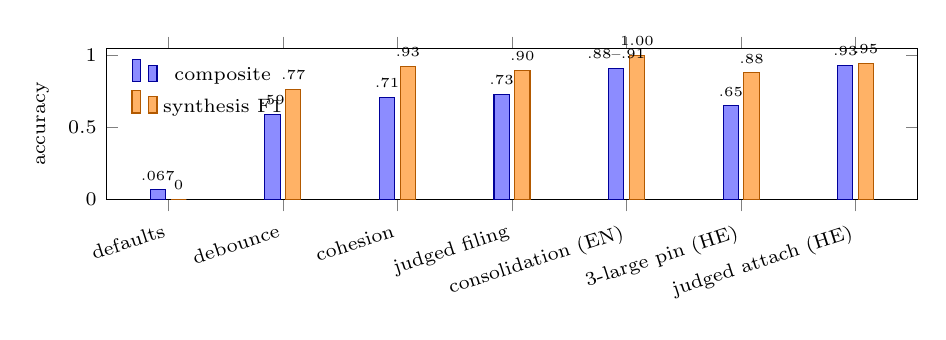
\begin{tikzpicture}
\begin{axis}[
  width=0.98\linewidth, height=3.5cm, ybar, bar width=5.5pt,
  ymin=0, ymax=1.05, ylabel={accuracy}, ylabel style={font=\scriptsize},
  symbolic x coords={defaults,debounce,cohesion,judged filing,consolidation (EN),3-large pin (HE),judged attach (HE)},
  xtick=data, x tick label style={font=\scriptsize, rotate=18, anchor=north east},
  y tick label style={font=\scriptsize}, legend style={font=\scriptsize, at={(0.02,0.97)}, anchor=north west, draw=none, fill=none},
  enlarge x limits=0.09, nodes near coords, nodes near coords style={font=\tiny}, point meta=explicit symbolic
]
\addplot[fill=blue!45, draw=blue!60!black] coordinates {(defaults,0.067)[.067] (debounce,0.592)[.59] (cohesion,0.711)[.71] (judged filing,0.730)[.73] (consolidation (EN),0.910)[.88--.91] (3-large pin (HE),0.651)[.65] (judged attach (HE),0.932)[.93]};
\addplot[fill=orange!60, draw=orange!70!black] coordinates {(defaults,0.000)[0] (debounce,0.765)[.77] (cohesion,0.926)[.93] (judged filing,0.895)[.90] (consolidation (EN),1.000)[1.00] (3-large pin (HE),0.880)[.88] (judged attach (HE),0.947)[.95]};
\legend{composite, synthesis F1}
\end{axis}
\end{tikzpicture}
\caption{The live-benchmark arc, as cumulative configurations at shipped thresholds, English then Hebrew. The English headline is quoted as a range over three arrival orders.}
\label{fig:arc}
\end{figure}
\paragraph{Cross-generator test.} As a check that we had not tuned to our own corpus, an independent vendor's model authored a second corpus of the same design with harder geometry, where the best cosine-only F1 is 0.871. The judged pipeline scored a synthesis F1 of \hl{0.980 with precision 1.000 and no false merges}, beating the cosine ceiling by 11 points on a corpus its authors did not write. Its composite of 0.791 was dragged down by a topic F1 of 0.508, because that generator's domains genuinely overlap.


\section{Two further hazards of a bare LLM}
\label{app:llmhazards}
\emph{Non-determinism.} At temperature zero the models are still not deterministic \citep{atil2024llm}. A sweep asked to find merge groups in a settled, correct set of ten headings proposed a wrong merge in one sample out of two. Production asks that question about 144 times a day, and a merge that any single call rarely proposes becomes, over enough calls, nearly certain (\S\ref{sec:convergence}).

\emph{Prompt sensitivity.} With the architecture held fixed, a plausible hand-written judge prompt scored 36\% on the hard triplets with 43\% false merges, where the production prompt scored 79\% and 7\% (App.~\ref{app:prompts}); only an adversarial test set makes such a gap visible \citep{sclar2024quantifying}.


\section{Cost and latency}
\label{app:cost}
Embeddings cost a rounding error next to completions. The registry classifier costs about \$0.11 per thousand classifications at small codebooks and about \$0.41 at codebooks of a hundred claims. The full engine, in corpus replay, averaged 2.85 calls per statement, about \$0.2--0.5 per thousand statements, at one to two seconds per placement and eight to ten seconds when the writer is consulted. The verdict cache and miss-billed budgets are not optional at scale. The sweep incident mentioned above cost about 3{,}100 completions a day on questions nobody was touching; after the fix, the same 21 refusals per tick that had spanned 46--52 seconds spanned about one second. The one path that remains unbounded is a burst of per-arrival triggers, and it fails closed: a duplicate stays visible, and nothing merges wrongly.


\section{Preference geometry and propositional equivalence}
\label{app:bpt}
The two tasks are siblings, not twins. \bpt model \emph{preferential similarity}: would the same participant endorse both statements? Our merge relation is \emph{propositional equivalence}: are these the same proposal? The two coincide on hard triplets, which is what licenses the shared benchmark, and they diverge elsewhere. Two distinct proposals can be preferentially similar, since a voter who wants speed bumps probably also endorses lower speed limits, and we must \emph{not} merge them, only theme them. Equivalence is binary and symmetric, so it fits a discrete codebook; preference is graded and relative to a participant, so it wants a geometry. One relation that neither geometry can carry is \emph{opposition}. ``Ban X'' and ``permit X'' are near each other in any topical space, and even a preference space encodes disagreement as distance rather than as claim and counter-claim. We store it as a typed edge, and that edge is what lets the interface show an idea together with its organised opposition.

Because our architecture confines geometry to candidate generation, their contribution slots in without redesign: a preference-tuned or per-topic-projected encoder is simply a better candidate generator. Today's cosine-ordered candidate lists are \emph{adversarially ordered}, with distractors outranking matches in 863 of 880 cases. A stance-faithful ranker should close the residual cross-lingual recall gap, shrink the gray zones and so cut judge calls, and exploit a signal we collect but do not use: the continuous evaluations on every statement, which their per-topic projection turns into a preference geometry from about fifty labelled triplets. What flows back is the decision layer. Their downstream problems still need statements deduplicated, labelled and synthesised first, and their own limitations section warns that the embedding should not ground binding decisions. Judged, audit-logged placement over a proposed geometry is one concrete answer to that warning, and the registry's \textsc{expresses} and \textsc{opposes} verdicts are, incidentally, the very triplets their tuning consumes, generated in-domain and for free.


\section{Documented failure modes and measurement discipline}
\label{app:failures}
\paragraph{The topic-cluster black hole.} In the first instrumented run one early topical cluster absorbed all 100 statements and no synthesis formed. The mechanism is general. In a corpus whose cosine floor is lifted, here by the shared question prefix, the first cluster created above the topical threshold becomes an attractor that every later statement clears, and if membership is terminal, every paraphrase pair is foreclosed. Coverage was 100\% while pair precision was 0.091. The fix was structural rather than a threshold: conjunctive cohesion gates, non-terminal topic membership, judged theme filing, and disabling theme creation from raw pairs. The black hole came back, instructively, when the Hebrew embedding model was upgraded without recalibrating the bands: a 45-member cross-topic theme formed, and 25 of its members entered through the one attach path that had no judge. Thresholds are properties of a geometry.

\paragraph{Snowballing.} Attaching on the best single member lets a synthesis grow by a chain of pairwise links until it spans several ideas. We measured it in production and again on the real-data replay, where an eight-member synthesis held six wrong members. The top-two member evidence, the centroid-and-quorum cohesion gate and the farthest-pair transitivity check in the sweep are the answers.

\paragraph{Silent drops in the streaming path.} A fifteen-second spawn debounce keyed per question suppressed spawns for unrelated pairs, so that 45 attempts became 24 spawns and 21 drops, and pair recall was capped at 40\% although every pair sat inside the attach band. A spawn that failed after the gate left no audit row and no retry. Both are instances of one shape, a suppressed action with no custodian, and both fixes are re-enqueues.

\paragraph{Order of passes.} Theming before synthesis let the general claim win on the specific claim's evidence: 17 of 23 topical attachments were justified by the statement's own twin. Most-specific-first fixed it.

\paragraph{Looping a non-deterministic judge.} A scheduled sweep asked to find merge groups in a settled, already-correct set of ten headings proposed a wrong merge in one of two samples, and production would have asked about 144 times a day. Each distinct set is now judged once, keyed on a fingerprint.

\paragraph{Replaying on end states predicts nothing.} An offline replay of the consolidation judge on each run's \emph{final} theme set predicted a clean reduction from 11 headings to 10. Live, the sweep met 19 half-formed headings and merged nine in one pass, and the run scored worse. A later reconstruction from full before-and-after membership snapshots showed that the impurity had entered at \emph{filing}, not at consolidation, in every run, so the original revert had been decided on confounded evidence. A decision must be evaluated on the states it actually meets.

\paragraph{Measurement that fails toward plausibility.} A harness that \emph{re-implemented} the production merge sweep kept measuring its own copy after the production code gained a judge gate. A settle detector's quiet window could not tell ``queued'' from ``finished'', and it reported 47 of 50 for a run that had achieved 50 of 50. Neither produced an error; both produced a number. Our response is a reproducibility discipline we commend to anyone benchmarking a live pipeline: import the production functions unmodified, certify builds byte for byte before and after each run, require two consecutive quiet windows and an unchanged double export, and mark contaminated runs ``do not cite'' rather than dropping them.

\section{Theme filing: the 2$\times$2 and the decision rule}
\label{app:filing}
On 58 judged filing decisions reconstructed to their exact live contexts, with three repeats each on the live model, the variants were: F0, titles with a prefer-file bias, which shipped at the time: 66.1\% accuracy, 28 misfiles, 31 over-refusals; F1, contents with prefer-file: 64.4\%, 37, 25; F2, contents with unsure-means-NONE: 62.6\%, 17, 48; F3, titles with unsure-means-NONE: 39.7\%, 15, 90; F4, contents with conflict-means-NONE: 70.1\%, 30, 22; F5, contents with NONE plus a narrowness exception: 71.8\%, 23, 26. The registered rule, minimise three times the misfiles plus the over-refusals with a hard cap of 19 misfiles, selects F2. F4 and F5 raise accuracy by re-licensing misfiles and fail the cap. Live confirmation: misfiles fell from 12 to 5, from 20.7\% to 9.3\%, with per-decision accuracy flat, and the reversible errors were then actually repaired by the sweep, which merged 13 donor headings, 12 of them same-topic.

\section{Text fidelity}
\label{app:fidelity}
A synthesis replaces what two people wrote with wording a model produced, and every membership metric would read 1.000 for a merge that held the right two members and published a proposal carrying only one of them. A validated fidelity judge, self-tested on five hand-written merges with known answers, grades each member as preserved, weakened or lost, and flags scope inflation and added commitments. Scoring titles only, fidelity ran 0.84--0.92 with no member lost across 300 member statements in three runs. Scoring the full text produced by the real compiled writer, fidelity was 0.990 with 4 of 50 scope inflations. Their cause was a contradiction inside the prompt, which forbade inventing facts while ordering the writer to state who does what on what timeline. Making that instruction conditional on the inputs and giving scope its own prohibition took inflation to 0 of 50 and fidelity to 1.000 with no new refusals. On the real-data replay, fidelity moved from 0.647 to 0.953 after the writer clauses.

\end{document}
